\section{Interazione e Comunicazione}
La comunicazione è uno dei punti cruciali del progetto,
sia per la quantità di informazione scambiata,
che per la sincronia dei messaggi.

\begin{figure}[H]
\centering
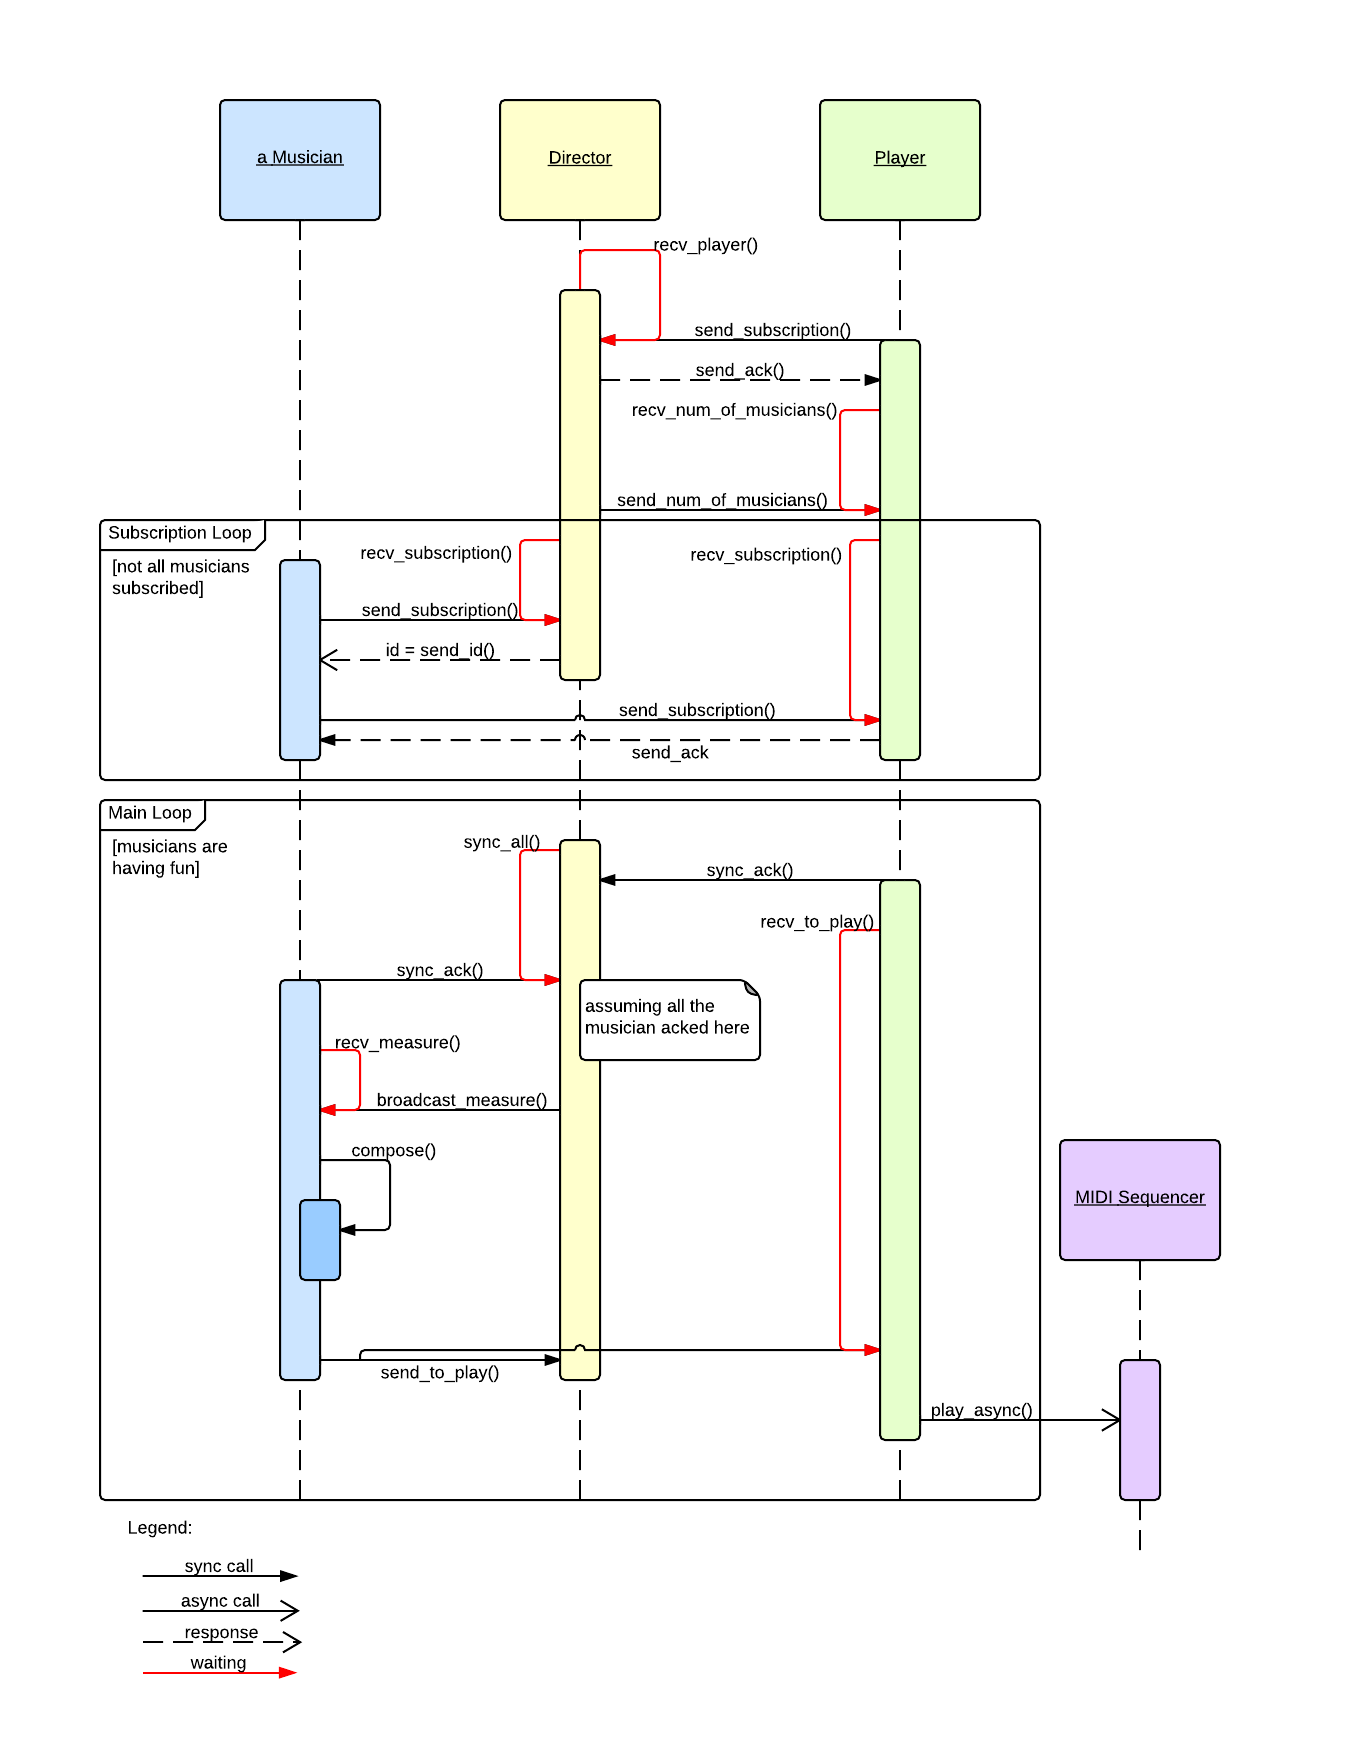
\includegraphics[scale=0.6]{img/protocol.png}
\caption{Diagramma del protocollo di comunicazione}
\end{figure}

Il protocollo è strutturato principalmente in tre fasi distinte.

\subsection{Inizializzazione}
Inizialmente il direttore riceve una sottoscrizione da parte del player.\\
Alla sottoscrizione (opportunamente segnalata tramite \emph{ack}), susseguirà un
pacchetto contenente il numero di musicisti
\footnote{In modo da specificare solamente al direttore
	  il numero di istanze di musicisti.}.
A questo punto l'inizializzazione dei componenti principali
(direttore e player) è completa, e la loro comunicazione, come vedremo
si limiterà a messaggi di sincronizzazione.

\subsection{Ciclo di Sottoscrizione}
A questo punto, ogni musicista si preoccuperà di inviare la sua sottoscrizione
all'improvvisazione sia al direttore che al player, in questo modo le due
componenti principali avranno una chiara visione dell'improvvisazione, pur
rimanendo completamente indipendenti.

\subsection{Ciclo principale}
Finita l'inizializzazione inizia il ciclo vero e proprio d'improvvisazione;
una volta sincronizzati tutti i musicisti (e il player) a barriera,
vengono inviate da parte del direttore le informazioni di improvvisazione,
come vedremo più avanti questi pacchetti contengono tutte le informazioni
sullo stato dell'improvvisazione, in modo da mantenere una certa coerenza
tra tutti i musicisti.\\
\\
Una volta composto, i musicisti inviano quindi la loro creazione
\footnote{Si rimanda alle opportune sezioni per approfondire come queste decisioni vengano prese.}
 al
player, il quale si occuper\'a di suonare la composizione nell'ordine corretto;
Mentre il direttore si occuper\'a della sincronizzazione, proseguendo con
un nuovo passo del ciclo.

\subsection{Libreria di comunicazione}
L'implementazione della libreria di comunicazione è presente nei file
\emph{communication.cpp} e \emph{struct.h}, se ne descrivono di seguito
i dettagli.

I principali pacchetti scambiati tra le varie istanze sono di 3 tipi:
\emph{Sottoscrizioni}, \emph{Misure} e \emph{Play Measures}.

\subsubsection{Sottoscrizioni}
Sono i pacchetti scambiati per la registrazione presso il Direttore o il Player
\begin{center}
\begin{bytefield}[bitwidth=1.1em]{32}
\bitheader{0-31}\\
\bitbox{32}{coupling}\\
\bitbox{8}{instrument\_class} & \bitbox{8}{flags}
\end{bytefield}
\end{center}

Essi contengono:
\begin{description}
\item[Coupling] \hfill \\
Un indicazione (per il player) sul fatto che il musicista sia in realtà una
composizione di più musicisti
\footnote{Immaginiamo ad esempio la mano sinistra e la mano destra dello
	  stesso pianista, le quali devono essere assegnate allo stesso
	  canale di output.}
\item[Instrument Class] \hfill \\
Il tipo di strumento, utilizzato per la ricerca nel database e per l'assegnamento
del corretto strumento \emph{MIDI} in uscita.
\item[Flags] \hfill \\\
I flag disponibili per la sottoscrizione sono:
\begin{itemize}
\item 0x0: Nessun flag rilevante.\\
\item 0x1: Il musicista è un solista.\\
\item 0x2: Il musicista utilizza pratiche di machine learning genetiche.\\
\end{itemize}
Da qui in poi sono riservati per utilizzi futuri.
\end{description}

La risposta a questi pacchetti non si limita al semplice ack, bensì ad
un pacchetto contenente l'id (univoco per la sessione) del musicista.\\

\'E necessario indicare che la registrazione del player presso il direttore
avviene inviando questo pacchetto con un coupling pari ad un valore costante
(-1).

\subsubsection{Misure}
Sono i pacchetti contenenti l'informazione sullo stato dell'improvvisazione
e il prossimo passo d'improvvisazione, sono inviati in broadcast dal direttore
a tutti i musicisti.

\begin{center}
\begin{bytefield}[bitwidth=1.1em]{32}
\bitheader{0-31}\\
\bitbox{8}{bpm}\\
\bitbox{32}{soloist\_id}\\
\bitbox{8}{tempo.upper} & \bitbox{8}{tempo.lower}\\

\begin{rightwordgroup}{9}
\bitbox{32}{prioargs}
\end{rightwordgroup}\\

\begin{rightwordgroup}{tempo.upper}
\bitbox{16}{note} & \bitbox{16}{scale}
\end{rightwordgroup}\\

\begin{rightwordgroup}{tempo.upper}
\bitbox{16}{chord} & \bitbox{16}{mode}
\end{rightwordgroup}\\

\bitbox{32}{tags length}\\
\bitbox{32}{tags (variable)}
\end{bytefield}
\end{center}

\begin{description}
\item[BPM] \hfill \\
Un indicazione sui bpm dell'improvvisazione corrente.
\item[Soloist ID] \hfill \\
L'ID del musicista che improvvisa correntemente in modalità solista.
\item[Tempo (upper e lower)] \hfill \\\
Indica la \emph{Time Signature} dell'improvvisazione corrente.
\item[Prioargs] \hfill \\\
Sono 9 campi costanti il quale compito \'e specificare
una scala di priorità con la quale effettuare le scelte di improvvisazione.
\footnote{Per una spiegazione pi\'u dettagliata si rimanda ai capitoli sul come
	  operano il  Direttore e il Musicista.}
\item[Note e scale] \hfill \\
Sono $tempo.upper$ campi contenti la successione dei centri tonali della misura (rilevanti per il solista).
\item[Chord e mode] \hfill \\
Sono $tempo.upper$ campi contenti la successione di accordi della misura (rilevanti per gli accompagnatori).
\item[Tags] \hfill \\\
\'E un campo testuale utilizzato per indicare attributi del pezzo da improvvisare
(è una terna che specifica genere, dinamiche ed intenzione).
\end{description}

\subsubsection{Play Measures}
Sono i pacchetti contenenti l'informazione dettagliata sulle note suonate
e la composizione che, in output dal musicista, viene passata al player
pronta per essere allineata con le altre battute ed essere suonata.

\begin{center}
\begin{bytefield}[bitwidth=1.1em]{32}
\bitheader{0-31}\\

\bitbox{32}{id}\\
\bitbox{32}{size}\\
\bitbox{32}{musician id}\\
\bitbox{8}{unchanged fst}\\
\begin{rightwordgroup}{Notes (size)}
\bitbox{8}{note.tempo} & \bitbox{8}{note.id} & \bitbox{8}{note.triplets} & \bitbox{8}{note.velocity} \\
\bitbox{8}{note.chord\_size}\\
\wordbox[lrtb]{2}{note.notes}
\end{rightwordgroup}\\

\bitbox{8}{bpm}\\
\end{bytefield}
\end{center}

\begin{description}
\item[Id] \hfill \\
Un numero progressivo (per musicista) indicante la posizione della battuta da suonare.
\item[Size] \hfill \\
Il numero di note presenti nella misura corrente.
\item[Musician id] \hfill \\\
L'identificativo univoco del musicista che ha generato la misura in questione.
\item[Unchanged fst] \hfill \\\
Un booleano indicante il fatto che la prima nota sia cambiata o meno.
\footnote{Questa feature \'e necessaria nel per effettuare dei legati
	  o dei continui dalla misura precedente.}
\item[Note] \hfill \\
Sono quindi presenti $size$ strutture contenenti le seguenti informazioni
\begin{description}
\item[Tempo] \hfill \\
La durata della nota (in sedicesimi).
\item[ID] \hfill \\
Un numero progressivo (per misura) indicante la posizione nella misura.
\item[Triplets] \hfill \\\
Un indicazione sul fatto che la nota debba essere scandita con tempo terzinato.
\item[Velocity] \hfill \\\
La velocity \emph{MIDI}, \'e un indicazione sul volume della nota in output.
\item[Chord\_size] \hfill \\\
Il numero di note presenti (nel caso sia un accordo,
altrimenti la nota sarà singola)
\item[Notes] \hfill \\\
Il vettore di note (in notazione \emph{MIDI}).
\end{description}
\item[BPM] \hfill \\
Un indicazione sui bpm da utilizzare nella riproduzione dell'improvvisazione.
\end{description}

\subsection{Meccanismi di sincronizzazione}
L'ultimo compito della libreria di comunicazione è
provvedere ad alcuni meccanismi per la sincronizzazione dei vari componenti.\\
Questo obiettivo è raggiunto utilizzando le chiamate di sistema di linux basate
sugli eventi quali \emph{epoll}: vengono radunati su di una barriera
(in qualsiasi ordine) tutti i musicisti, dopo di che viene notificata, tramite
\emph{ack}, la possibilità di continuare.
